\documentclass[a4paper]{article}
\usepackage[utf8]{inputenc}
\usepackage[T1]{fontenc}
\usepackage{graphicx}
\usepackage{hyperref}
\usepackage[english]{babel}
\usepackage[super]{nth}
\usepackage{fancyhdr}
\usepackage{tabu}
\usepackage{multirow}
\usepackage{cite}
\usepackage{amsmath}


\newcommand*\mean[1]{\overline{#1}}

\DeclareGraphicsExtensions{.pdf,.png,.jpg,.eps}

\newcommand{\myauthor}{TODO Names of Authors}
\newcommand{\mytitle}{Zombie Apocalypse Report}

\lhead{\mytitle}
\rhead{\myauthor}

\pagestyle{fancy}
\fancyhf{}
\fancyhead[L]{TODO names of authors}
\fancyhead[R]{\mytitle}

\fancyfoot[C]{\thepage}

\title{\mytitle}
\author{\myauthor}

\begin{document}
\maketitle

\section{Introduction} % Ryan

Infectious diseases have been prevalent since the start of time. Modelling the spread of these diseases can serve to find a possible ways to stop or contain the spread. With the advancement of technology, computing power has increased tremendously, allowing these simulation models to be done on a greater scale. In this project, we are to implement a Zombie Infection simulation, modeling the spread of the infection on a human population. The entities in the simulation are split into three main categories, Humans, Infected and Zombies. Infected are humans which will eventually turn into Zombies. 

In the first part of this project, the task was to simulate the population on a 500 by 500 grid. We had take into account the birth and death rate of humans, keeping close to the current demographics of the Northern Territory in Australia. 

We also had to simulate zombie conversion, decay and movement. Since this is a, currently, fictional virus, the various different literatures have different zombie characteristics. In an article on the zombies of “World War Z”, the zombies in this lore are slow moving until they sense humans around. They will then move as fast, if not, faster than human running speed \cite{guidetozombies}. In this project, we set the zombie decay rate of 1 year (meaning that a Zombie would decompose after a year), which was adapted from \cite{zombiepedia}, had to also be taken into account. This meant that the zombies would die out without any humans to infected. These zombies naturally move towards the humans to infect them, converting humans into zombies. The gestation period for the infected humans to turn into zombies was also adapted from the same source. Movement also needs to be implemented correctly, as both humans and zombies have different speeds.

With this model, we aim to be able to simulate an actual infection, by modeling a stable population of both humans and zombies, finding the right distribution for both to coexist. 

\section{Model} % Adam

\subsection{Infection model}

\begin{figure*}[ht]
        \centering
        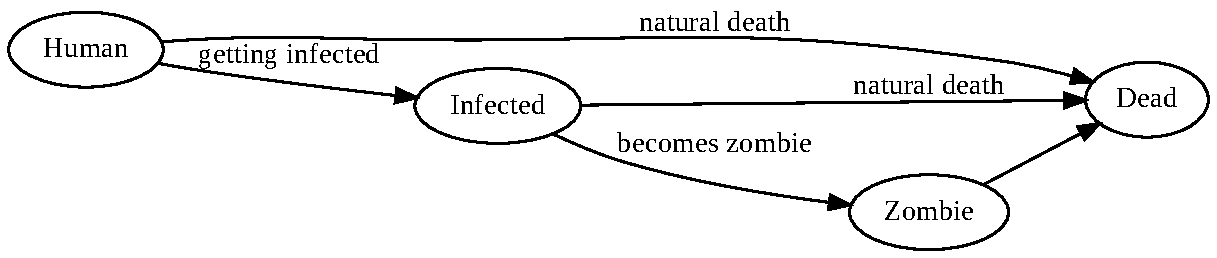
\includegraphics[width=\textwidth]{model}
        \caption{Infection model}
\end{figure*}

Since there has not been found cure for zombies to become humans, our model presumes only four possible stages.
An entity begins in state Human which represent a normal human being which was born, has a gender (is either male of female) and eventually dies.
If a human gets in contact with a zombie, it may become infected.
Infected entity is basically a human which eventually becomes a zombie which means that it can reproduce and die of natural death.
Infected entity is not a danger to the surrounding humans until it becomes a zombie.
When in contact with a human, a zombie may infect him or her.
Zombie is concidered death -- it is just a virus driven moving body; therefore we say that a zombie eventually decomposes insead of it dies.
In our model, zombie doesn't have gender as it cannot reproduce nor its properties depend on gender of the human which it used to be.

When a human becomes infected, the length of the infection is determined by the strength of the body fighting zombie virus.
The virus seems to be latent once a day it tries to gain control over the body.
It will happen with a certain probability.

\subsubsection{Reproduction}

If two fertile living entities (no matter if human or infected) of different genders meet, they can make love and conceive a child or children.
It takes approximately 9 months for the children to develop inside mother's womb before they are born.
As the zombies are of viral nature, we presume that the virus in infected mother's body is passed to unborn children.
The virus is not transmitted when an infected has an intercourse with a human.

A woman can become pregnat if she is not already pregnant and she is an a fertile age (roughtly between 15 and 45 years) and her partner is a male in a fertile age (roughtly between 15 and 80).
More than one baby can be conceived during one intercourse -- our model supports that a female can have up to three children at once.
The probabilities of multiple births are in accordance with Hellin's law. (TODO reference)

\subsubsection{Age}

The model follows the Australian age distribution for both males and females.
When the simulation starts, the people are didided into age classes based on their gender.
Within the age class the people are distributed uniformly.

Humans and infected are sorted into four age classes:
\begin{enumerate}
\item a child (0 -- 15 years)
\item young (15 -- 37.5 years)
\item middle aged (37.5 -- 65 years)
\item elderly (54 -- $\infty$)
\end{enumerate}

According to latest scientific research (TODO reference), zombies live 3 to 5 years. 
Zombies are divided into two age classes:
\begin{enumerate}
\item young (0 -- 1.5 years)
\item old (1.5 -- $\infty$)
\end{enumerate}

Most of the properties of the entities are dependent on their age class rather than on their actual age.
Those properties are:
\begin{itemize}
\item daily death rate -- probability of natural death per each day
\item speed -- probability of entity to leave current tile if it was its original intension
\end{itemize}

We have good estimates for living entities, but we are still waiting for our colleagues to determine the values for zombies depending on their age.

\subsection{World representation}

The simulated world is a mesh of size $1000 \times 1500$ which correspond with size of Northern Territory. (TODO reference)
Parts of the mesh are called tiles.
On each tile, there may be at most one entity of any type.
Adjacency of two entities means that the two entities are touching each other, sharing one side of their tiles.
The simulated world has fixed boundaries and no entity can pass through them; this is often refered as no-flux boundary. (TODO reference)

For the purpose of this report, only part of the world is simulated.
The actual size of the mesh is $500 \times 500$ tiles.

\subsubsection{Movement}

\begin{figure*}[ht]
    \centering
    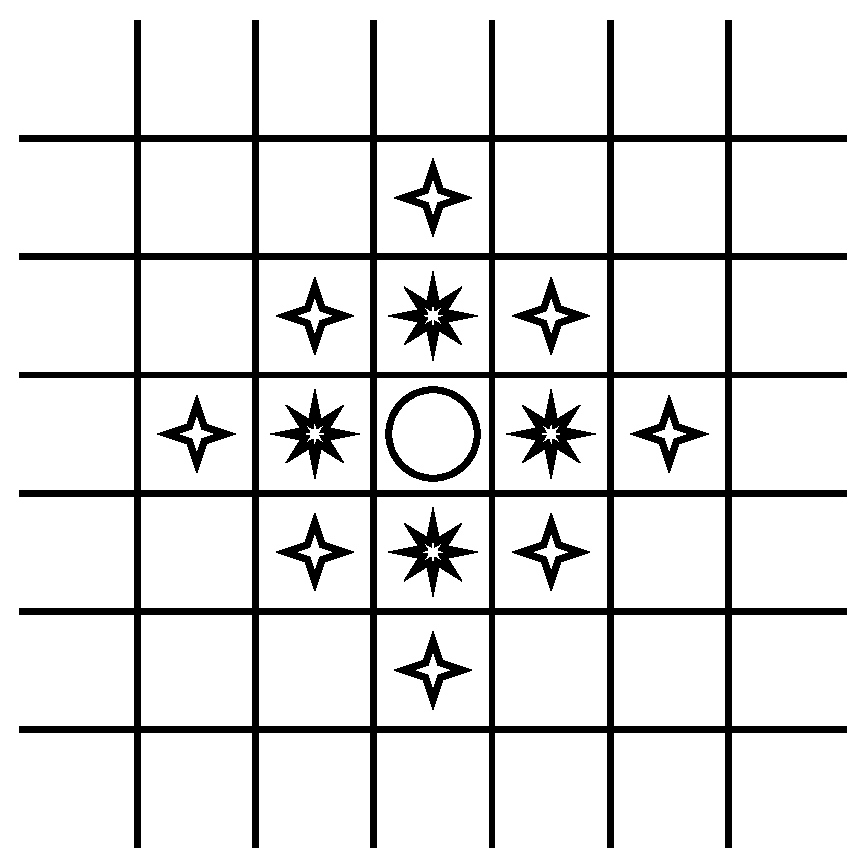
\includegraphics[width=0.3\textwidth]{movement}
    \caption{Considered tiles when planning movement}
\end{figure*}

\begin{figure*}[ht]
    \centering
    \begin{tabu} {| X[1.8,c,p] || X[1,c,p] | X[1,c,p] | X[1,c,p] | X[1,c,p] | X[1.2,c,p] |}
        \rowfont{\bfseries}
        \hline
        sees &
        Wall &
        Empty tile&
        Zombie &
        Same gender &
        Opposite gender \\
        \hline
        \hline
        \textbf{Living entity} & -- & + & -- & + & ++ \\
        \hline
        \textbf{Zombie} & -- & + & + & \multicolumn{2}{c|}{ ++ } \\
        \hline
    \end{tabu}
    \caption{Affinity to directed situations for each type}
\end{figure*}


All entities share the same intelligence, even zombies.
They differ mainly in preference where to go.

Each entity determines its optimal direction based on surrounding 12 tiles as shown on the diagram.
The tiles which it can get within one move are marked with a fancy star; tiles accessible within two moves are marked with a simple star.
The adjacent tiles always have higher priority.

Each living entity and zombie rate each of these tiles based on their content.
The preference for direction is then calculated as a weighted sum of complex numbers corresponding to direction.
The exact values of preferences may change as soon as we obtain a broader set of observations of entities in various situations.
However the estimates can be seen in the table.
To the current preffered direction the direction from the last move is added, which simulates inertia of movement and as a result it makes the movement targeted.

After the optimal weighted direction is calculated, it is translated to a direction or stay instruction if the absolute value is not sufficient.
The direction may randomly change clock-wise or counter-clock-wise simulating evading obstacles, which are not modeled in the world.
Then the tile in resulting direction is tested whether it is free; if it is not, the clock-wise or cunter-clock-wise is chosen.
In the worst case, the entity stays at its current tile.
The entity moves only if its speed (expressed as probability) is sufficient.

\subsection{Initialisation of the population}

\subsubsection{Age structure and death rate}

\begin{figure*}[ht]
    \centering
    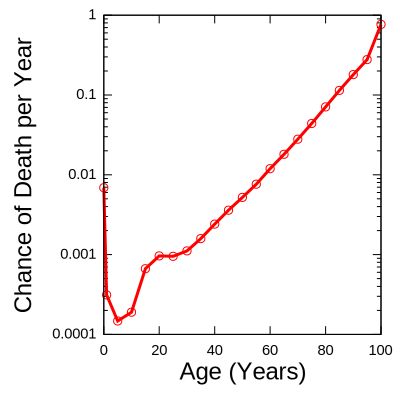
\includegraphics[width=0.6\textwidth]{USGompertzCurve}
    \caption{Mortality rates graph for US in 2003}
\end{figure*}

According to Australia age structure\cite{agestructure} and median age 37.3\cite{demographicsaustralia}, initialized human are divided into four age classes, named child (0-15 years old), young (15-37.5 years old), middle age (37.5-65 years old) and elder (above 65 years old) in the program.
Based on Gompertz–Makeham law\cite{mortalitylaw} and mortality rates graph for US in 2003 (shown in the figure) the average probabilities of human dying at these four age stages are approximately related as 
$$ \mean{P(\text{Elder Death})} = 10\: \mean{P(\text{Middle Age Death})} $$
$$ = 80\: \mean{P(\text{Young Death})} = 160\: \mean{P(\text{Child Death})} $$

As Australia death rate\cite{absdeath} is
$$ \mean{P(\text{Australia Death})} = \frac{\text{people dead (in 2012)}}{\text{population (in 2012)}} $$
$$ = \frac{147098}{23319400} = 0.63\%/\text{year} = 0.0017\%/\text{day} $$

The death rate of each age class can be calculated out as the table shown below:

\begin{figure*}[ht]
    \centering
    \begin{tabu} {| X[1.1,c,p] || X[0.7,c,p] | X[1.2,c,p] | X[1.1,c,p] | X[1,c,p] |}
        \rowfont{\bfseries}
        \hline
        Class Name &
        Age Range &
        Distribution &
        Average Death Rate (per day) &
        Death Rate (per day) \\
        \hline
        \hline
        \textbf{Child} & 0--15 & 18.2\% & \multirow{4}{*}{0.0017\%} & 0.00006\% \\
        \cline{1-3}\cline{5-5}
        \textbf{Young} & 15--37.5 & 31.8\% & & 0.00012\% \\
        \cline{1-3}\cline{5-5}
        \textbf{Middle Age} & 37.5--65 & 35.6\% & & 0.00096\% \\
        \cline{1-3}\cline{5-5}
        \textbf{Elderly} & 65+ & 14.4\% & & 0.0096\% \\
        \hline
    \end{tabu}
    \caption{Death rate of age classes}
\end{figure*}

\subsubsection{Birth rate}

The Australia birth rate is\cite{absbirth}:
$$ P(\text{Australia Birth}) = \frac{\text{baby birth}}{\text{population}} = \frac{158988+150594}{23319400} = 1.33\% $$

To achieve this birth rate when the world is simulated, some initialized women should be pregnant at this stage.
If female fertility period is from 15 to 45, then women in genital stage is 41.5\%.
Thus in initialization stage, pregnancy probability of women who is in fertility period is: 
$$ P(\text{Pregnant Women in Fertility Period}) = \frac{\text{baby birth}}{\text{women population} \times 41.5\%} $$
$$ = \frac{158988+150594}{11659700 \times 41.5\%} = 2.655\% $$

\subsubsection{Sex ratio}

There were 102,300 more females than males residing in Australia in 2012, with 11.3 million males and 11.4 million females.\cite{abspopulation}
Thus the sex ratio is initialized as 
$$ \text{Female} : \text{Male} = 0.502 : 0.498 $$

\subsubsection{Population Density}

The population density in Northern Territory prior to the zombie apocalypse was $0.17/\text{km}^2$. \cite{northernterritory}
When the viral infection started, approximately half of the population left Australia to Sweden. \cite{project}
As the simulated mesh is $500 \times 500$, the number of simulated people is
$$ 500 \cdot 500 \cdot \frac{0.17}{2} = 21250 $$

\section{Results}

TODO two images of state and a graph of populations' count.

\subsection{Demographics}

TODO demographics during the simulation.
Unfortunately we haven't implemented a function which prints information about individual people -- gender + age.

\subsection{Scaling}

\begin{figure*}[ht]
    \centering
    \begin{tabu} {| X[0.8,c,p] || X[1,c,p] | X[1,c,p] | X[1,c,p] |}
        \rowfont{\bfseries}
        \hline
        Threads &
        First attempt &
        Second attempt&
        Third attempt \\
        \hline
        \hline
        \textbf{1} & 180588.734000 & 180633.477000 & 180441.396000 \\
        \hline
        \textbf{2} & 94541.958000 & 95547.356000 & 94704.053000 \\
        \hline
        \textbf{4} & 49689.704000 & 50052.682000 & 50359.165000 \\
        \hline
        \textbf{8} & 25863.988000 & 26373.077000 & 26276.703000 \\
        \hline
        \textbf{16} & 14365.825000 & 14386.286000 & 14363.556000 \\
        \hline
        \textbf{32} & 10598.242000 & 10936.435000 & 10854.121000 \\
        \hline
        \textbf{64} & 14785.381000 & 14363.065000 & 14936.496000 \\
        \hline
    \end{tabu}
    \caption{Scaling depending on number of threads}
\end{figure*}


The model implemented in C using OpenMP can utilise several threads.
On Avoca the IBM Blue Gene/Q supercomputer, a single node provides 16 cores with 4 threads each.
Our model could utilise all 64 threads as most of the simulation does not need any thread synchronisation.

We run the model three times for 1000 iterations in order to ensure the influence of randomness does not make the results odd.
The results are in the table above, running times are in milliseconds.
We expect a perfect scaling up to 16 threads -- each of them will be assigned to a dedicated core.
Running with 32 cores still provides an improvement but not a significant one.
The drop of performace when running with 64 threads is either caused by the hardware architecture of the CPU or by using wrong random generators.
In our opinion it is not caused by locking parts of the world as there are still at least 7 columns for each thread (we lock only three of them).

\section{Recommendations}

Due to the large initialized population density and birth rate which is greater than average death rate, the human population will keep growing for a few years until the zombie population is large enough to meet and infect the human in significant speed.
In this case, the infected population is much greater than the amount of new birth human.
So the human population will drop quickly and the zombie population will be at its peak.
However a zombie can only live for 3 years normally.
If the human population is too low, zombie who has no birth income will die out soon.
In addition, the more human in initialization stage, the sooner the world collapses.

\subsection{Uncontrolled birth}

Theoretically the world should start with 21250 human.
The flow diagram below shows a testing result of the world starting with only 8000 human and 2 zombies.
After about only 63 years, zombies died out and human population dropped to 1809 people.

\begin{figure*}[pht]
    \centering
    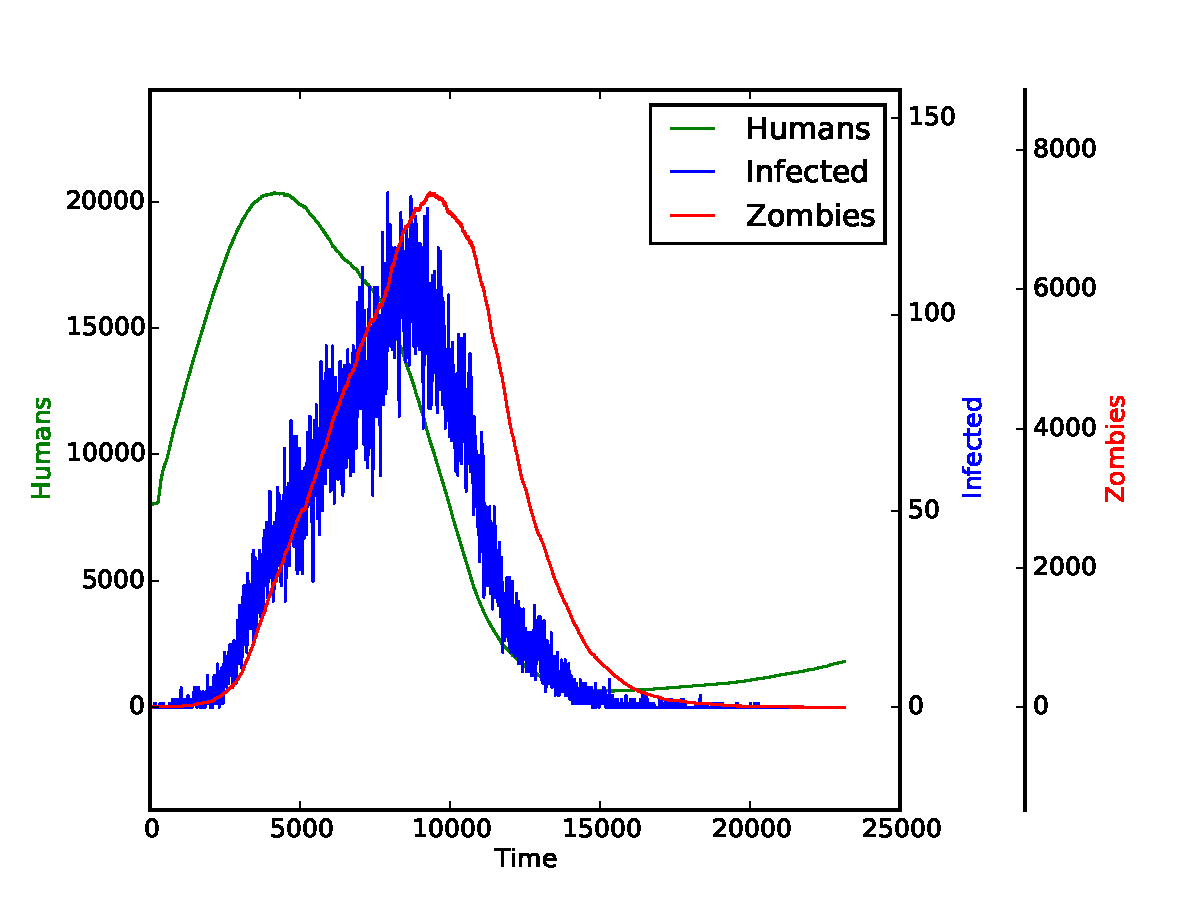
\includegraphics[width=\textwidth]{uncontrolled_birth_8000}
    \caption{Uncontrolled birth with 8000 people and 2 zombies}
\end{figure*}

\subsection{Equal birth}

In order to make sure that the world lasts forever, we assume that the human can self-control the human birth rate to avoid dying out for being infected by a large amount of zombies.
At the beginning, humans and infected calculate their dead and infected who become zombies, and set the birth rate to maintan current population.
Some pregnant females will be infected and become zombies so the human population will decrease.
The result of the model is in the figure.

\begin{figure*}[pht]
    \centering
    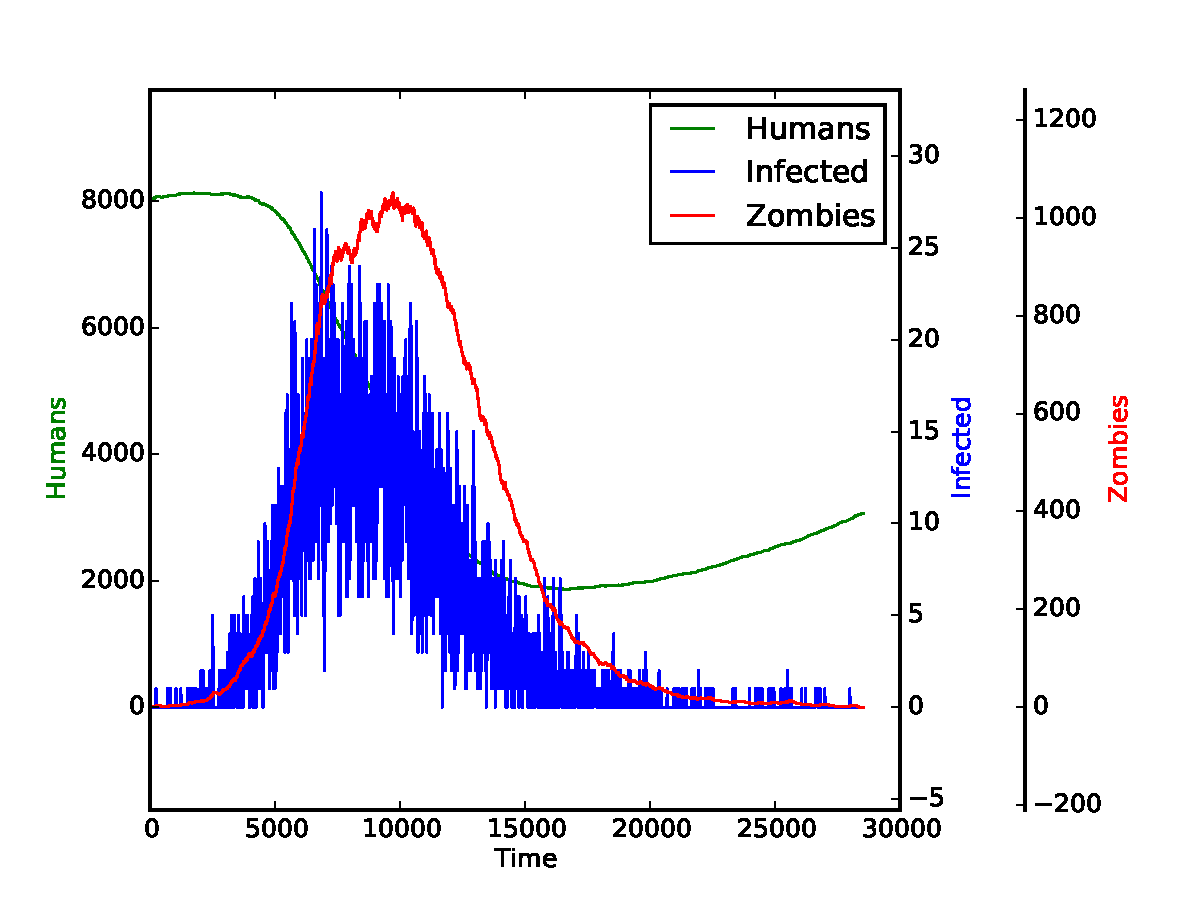
\includegraphics[width=\textwidth]{equal_birth_8000}
    \caption{Equal birth with 8000 people and 2 zombies}
\end{figure*}

\subsection{Stable population}

When the human population is under 12000, at the time when zombie and human populations are almost equal, the human will be alerted that they should have more babies otherwise they will die out.
As the human birth has a gestation period and the zombie population will drop down sharply due to the low human population and meet chance, human population will grow remarkably after 10 years. 
This way the human and zombie population gets to equilibrium as shown in the figure which shows 273 years of simulation.

\begin{figure*}[pht]
    \centering
    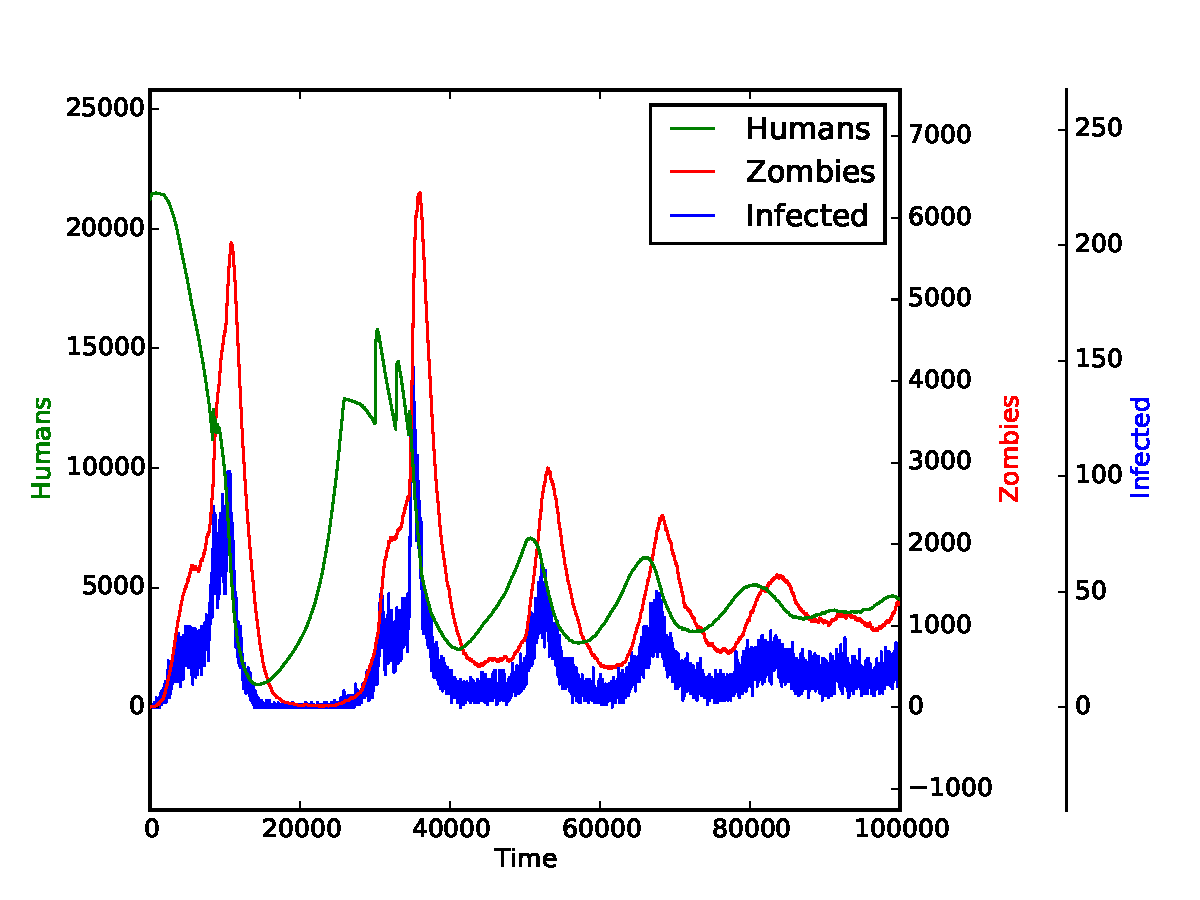
\includegraphics[width=\textwidth]{stable}
    \caption{Stable populations of humans and zombies}
\end{figure*}

As another test diagram of ten times longer simulation shown below, the change of populations of human, infected and zombie will follow the law of 40 years cycle.
The population swings are fewer and fewer.
And they are quite stable after 465 years.

\subsection{Real Recommendation}

In order to get to the equilibrium, we can recommend people to behave normally until their population drops one half.
Then they should stop using birth control (which as a human-made resource won't be available anyway) and start reproducing like rabbits.
This strategy ensures that the populations of both, humans and zombies, gets stable over time.

\begin{figure*}[pht]
    \centering
    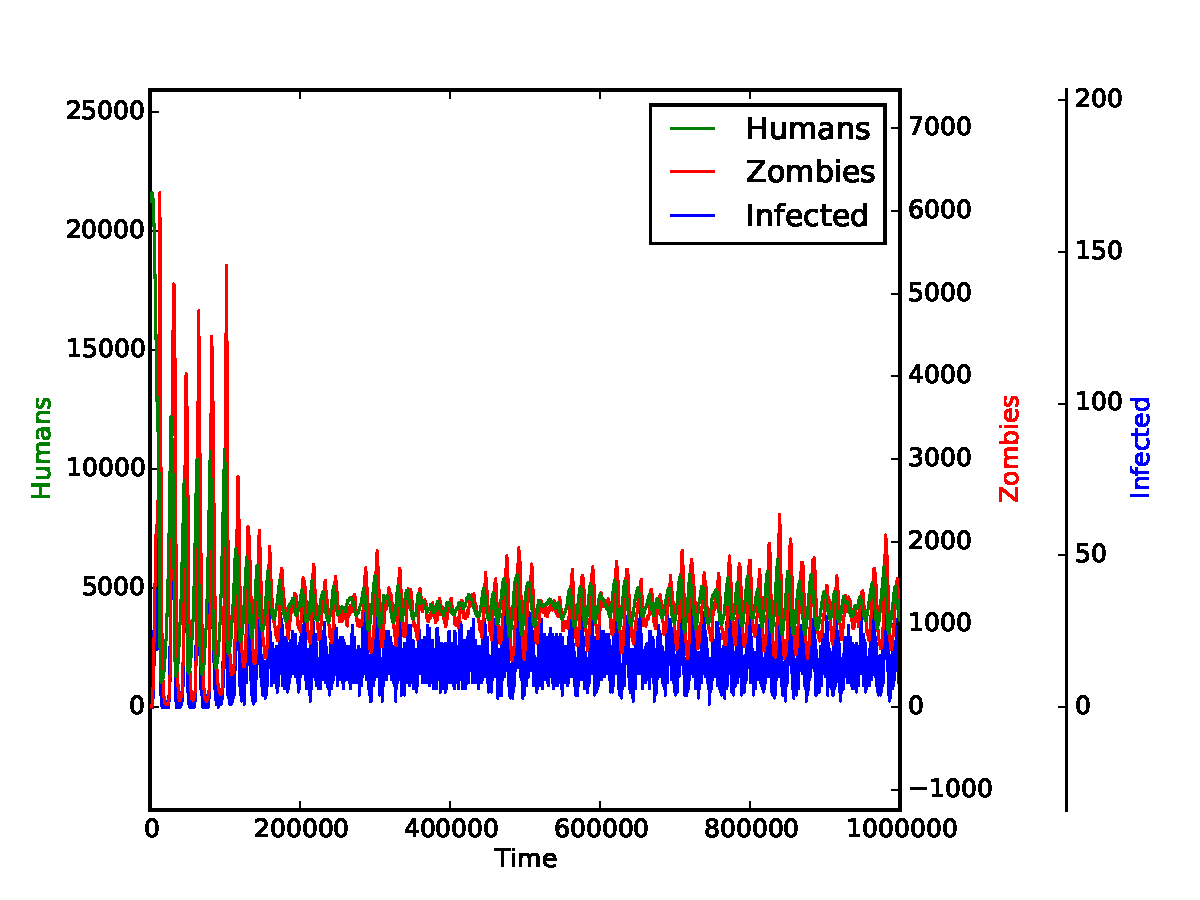
\includegraphics[width=\textwidth]{stable_1000000}
    \caption{2740 years long stable simulation}
\end{figure*}

\begingroup
\raggedright

\bibliographystyle{IEEEtran}
\bibliography{references}
\endgroup

\end{document}

% vim: ft=tex ts=4 sw=4 et
